\documentclass[10pt,twocolumn]{article}

\usepackage[utf8]{inputenc}
\usepackage{amsmath}
\usepackage{amssymb}
\usepackage{hyperref}
\usepackage{booktabs}
\usepackage{graphicx}
\usepackage{float}
\usepackage{placeins}
\usepackage{tikz}
\usetikzlibrary{arrows.meta,positioning,calc,backgrounds,fit}
\graphicspath{{figures/}}
\raggedbottom
\setlength{\intextsep}{6pt plus 2pt minus 2pt}    % gap above/below [H] floats
\setlength{\textfloatsep}{8pt plus 2pt minus 2pt}
\setlength{\dbltextfloatsep}{8pt plus 2pt minus 2pt} % for figure* (Fig 4, Fig 10)
\setlength{\floatsep}{6pt plus 2pt minus 2pt}
\setlength{\abovecaptionskip}{4pt}
\setlength{\belowcaptionskip}{2pt}

\title{\LARGE \textbf{Law as Code in Autonomous Drone Perception:\\ Active Inference for Context-Dependent Legal Compliance}}
\author{Mahault Albarracin \and Nicolás Hinrichs}
\date{2026}

\begin{document}

\maketitle

\begin{abstract}
Autonomous drones that perceive and act in real time create legal compliance problems that post-hoc auditing cannot fix: by the time a violation is detected, the drone has already acted. We propose a Legal Actuator Layer (LAL), a middleware between perception and actuation that enforces regulatory constraints before the drone acts. Where conventional Law-as-Code encodes rigid if-then rules, we formalize legal obligations as prior preferences in an Active Inference (AIF) agent that weighs competing obligations, such as privacy versus mission completion or geofence compliance versus emergency response, through expected free energy minimization. Nine simulation experiments using \texttt{pymdp} show that where a single obligation applies, the AIF-LAL matches the compliance of hand-coded rules: it reproduces the rule-based agent's GDPR data minimization exactly and respects EASA geofences with zero unjustified incursions. Where obligations conflict, it outperforms both rule variants: it enters restricted airspace during an authorized medical emergency that a rigid geofence rule misses entirely, while a rule with a hard-coded emergency exception, fed the same noisy dispatch signal, fires on noise in over half of normal trials. Comparisons against three baseline agents, a sensitivity sweep over the two main preference magnitudes, and an observation-noise sweep show that on the experimental condition where the legal trigger and the privacy constraint are out of phase, the AIF agent is the only one of the four that reaches the mission target on every trial while keeping privacy violations low, and that under heavy sensor noise it mostly stops acting, which keeps observation error from compounding into violations. A learning experiment shows that na\"ive Bayesian acquisition of the observation model collapses this behavior even though the learned model is close in $L^1$; calibrating the compliance-relevant sensors by hardware and learning only the environmental signals recovers full mission success and most of the lost compliance. The residual gap is itself informative: the channel that carries legal sanctions cannot be learned by an agent that complies, because generating the training data would mean violating. Inference cost on a single RTX 5070 GPU is $1148\,$ms per decision cycle in a Python-driven loop but drops to $0.31\,$ms ($3{,}260$ Hz) when the cycle is JIT-compiled through \texttt{jax.lax.scan}, more than two orders of magnitude below the $100\,$ms target.
\end{abstract}

%% ─────────────────────────────────────────────────────────
\section{Introduction}
%% ─────────────────────────────────────────────────────────

Autonomous drones equipped with computer vision make control decisions faster than any human operator can review~\cite{hildebrandt2015}. Each frame captured, each motor command issued, may violate privacy law, aviation regulation, or AI governance rules, yet the drone acts before any oversight is possible. Regulatory Technology (RegTech) addresses analogous problems in finance through retrospective monitoring~\cite{arner2017}, but a drone that has already followed a bystander into restricted airspace cannot undo the violation after the fact. Compliance must be enforced \textit{before} the drone acts, not after.

``Law as Code'' (LaC) addresses this need by translating legal rules into machine-executable constraints that restrict a system's behavior at runtime~\cite{diver2021, surden2012}. Existing LaC implementations, however, rely on deterministic rules that cannot handle competing legal obligations. A drone that always anonymizes video feeds to satisfy the GDPR will lose its surveillance target; one that never enters restricted airspace will abort every mission where a target crosses a geofence boundary. Legal reasoning is \textit{defeasible}: higher-priority obligations override lower-priority ones depending on context~\cite{prakken2015}. A medical emergency suspends privacy constraints, and an imminent collision overrides geofencing restrictions. A fixed rule set has no way to represent that one obligation gives way to another only under some conditions.

Several approaches address parts of this problem. Defeasible logic frameworks resolve conflicting legal rules through explicit priority orderings~\cite{prakken2015}. Constrained MDPs encode safety requirements as hard constraints on expected costs~\cite{garcia2015}. Rules-as-code languages such as Catala handle exceptions through built-in default logic~\cite{merigoux2021}. These approaches work well when the agent knows which context applies. A drone operating under uncertainty often does not: it may not know whether the person ahead is having a medical emergency, whether bystanders are in the scene, or whether it has crossed into restricted airspace.

We propose that AIF~\cite{friston2017, dacostaAIF2020, parr2022} addresses this gap. In AIF, an agent maintains a generative model of how hidden states cause observations and selects actions by minimizing expected free energy (EFE). Legal obligations can be encoded as prior preferences over observations, extending the active-inference treatment of social norms as priors over expected experience~\cite{constant2019}: GDPR data minimization becomes a preference for low \textit{biometric exposure} (the rate at which identifiable facial data of non-target persons is captured and transmitted), and EASA geofencing becomes an aversion to GPS readings inside restricted zones. Because preferences have magnitudes, higher-priority obligations (e.g.,~collision avoidance) override lower-priority ones (e.g.,~privacy) when they conflict. Unlike symbolic priority systems, the agent also infers its legal context from noisy observations and actively seeks information before committing to an action.

The paper contributes (i) an analysis of compliance gaps in a typical edge-AI drone architecture across three EU regulatory frameworks (Section~\ref{sec:gaps}); (ii) a formalization of the Legal Actuator Layer (LAL) at the perception-actuation boundary as an AIF agent whose preferences encode legal obligations through belief-weighted profile mixing (Sections~\ref{sec:lal}--\ref{sec:aif}); and (iii) nine simulation experiments characterizing where this AIF-LAL handles competing obligations rigid rule-based systems cannot, how it trades off mission success against compliance as sensors get noisier, and where it breaks (Section~\ref{sec:experiments}). The clearest limit is in the learning regime: a Bayesian agent that tries to acquire its full observation model from data loses the discrimination needed for emergency override. The fix, which we test, is to specify the legally relevant sensor channels by hardware calibration and learn only the rest. It recovers most of the lost compliance. The part it cannot recover points to a structural problem for any learned compliance system: a compliant agent never gathers the data that would teach it what sanctions look like.


%% ─────────────────────────────────────────────────────────
\section{Compliance Gaps in Edge-AI Drone Perception}
\label{sec:gaps}
%% ─────────────────────────────────────────────────────────

Micro-drones such as the DJI Tello lack the compute budget to run neural networks onboard. Developers therefore offload perception to a remote server, a pattern common in edge-AI deployments~\cite{zhou2019}: the drone captures and transmits video frames over HTTP, while a remote server runs inference via RESTful APIs. This architecture maps directly onto GDPR data-protection roles: the drone operator is the data controller, who determines the purpose of processing, and the server is a data processor that acts on the controller's behalf~\cite{gdpr2016}. Legal obligations must therefore be enforced at the network boundary. A typical implementation of this kind exhibits three categories of legal vulnerability.

\textbf{Data minimization.} The image-sender thread captures 720p frames from the drone's UDP video stream and transmits them as base64 over HTTP. Every bystander's face is captured and sent to the server regardless of whether that person is the tracking target, violating the data minimization principle of GDPR Article~5(1)(c)~\cite{gdpr2016}. Base64 is an encoding, not a cipher, so the transmission is unencrypted and biometric data is exposed to interception in violation of GDPR Article~32~\cite{gdpr2016}.

\textbf{Automated decision-making.} The control function converts bounding-box coordinates directly into motor commands. No human reviews the decision. Under the EU AI Act, biometric tracking in public spaces is classified as high-risk and requires human oversight (Art.~14) and event logging for traceability (Art.~12)~\cite{euai2024}. Typical implementations provide neither.

\textbf{Geofencing.} The PID controller tracks its target without any knowledge of where it is flying. If the target walks into restricted airspace, the drone follows, violating geofencing rules in EASA's U-space framework (the EU low-altitude unmanned-airspace regime) and visual-line-of-sight requirements~\cite{easa2019}.

All three problems have the same root cause: the control loop has no representation of legal context. The PID error signal,
\begin{equation}
    \text{Yaw} = K_p\,(x_{\text{center}} - x_{\text{target}}) + K_d\,\tfrac{d}{dt}(x_{\text{center}} - x_{\text{target}}),
\end{equation}
minimizes tracking error and nothing else. Whether the target is in a public park or restricted airspace, whether bystanders are present or absent, the controller behaves identically.


%% ─────────────────────────────────────────────────────────
\section{The Legal Actuator Layer}
\label{sec:lal}
%% ─────────────────────────────────────────────────────────

We propose inserting a Legal Actuator Layer (LAL) between perception and actuation. On the perception side, the LAL anonymizes non-target faces by face detection and irreversible blurring, all in volatile memory, before anything is transmitted. This implements privacy by design at the edge~\cite{cavoukian2009}. On the actuation side, it enforces geofencing constraints on motor commands and writes every decision to an append-only audit log. Each log entry records perception confidence, actuation vectors, and policy posteriors per cycle, which satisfies EU AI Act traceability requirements.

Enforcing any single rule is straightforward. The hard part is deciding what to do when rules conflict. If the LAL always blurs video, it may obscure obstacles and cause a collision. If it always respects a geofence, it may prevent the drone from reaching a medical emergency. Legal obligations have an implicit priority ordering: safety first, then emergency response, privacy, and mission objectives. The LAL must respect this ordering at runtime.

One could hard-code this ordering as nested if-then-else logic, but every new regulation or context variable multiplies the number of branches. We take a different approach: we formalize the LAL as an Active Inference agent, where the priority ordering falls out of the relative magnitudes of prior preferences in a generative model. The next section describes how.


%% ─────────────────────────────────────────────────────────
\section{Active Inference Formulation}
\label{sec:aif}
%% ─────────────────────────────────────────────────────────

We model the LAL as a Partially Observable Markov Decision Process (POMDP) with the standard Active Inference parameterization $(\mathbf{A}, \mathbf{B}, \mathbf{C}, \mathbf{D})$. $\mathbf{A}$ is the observation likelihood mapping hidden states to observations in each modality, $\mathbf{B}$ is the transition model $P(s_{t+1} \mid s_t, u_t)$, $\mathbf{C}$ is a vector of log-preferences over observations, and $\mathbf{D}$ is the prior over initial hidden states.

Legal constraints map directly onto $\mathbf{C}$. GDPR data minimization becomes a preference for observing low biometric exposure; EASA geofencing becomes an aversion to GPS readings inside restricted zones; EU AI Act traceability becomes a preference for maintaining an audit trail. We make $\mathbf{C}$ depend on \textit{inferred} context. Urgency and privacy status are hidden state factors that the agent must estimate from noisy observations. When the agent infers that an emergency is occurring, preference magnitudes shift: the drive toward the mission target rises from $-2$ to $+6$, the direct aversion to occupying the privacy zone relaxes from $-6$ to $0$, and the complaint aversion that normally prevents crossing falls from $C_3 = [8, -8]$ to $[1, -1]$ (Section~\ref{sec:experiments} gives the full profiles). The EFE computed over all observation modalities then favors advancing. Nothing in this is a rule that switches on: the ordering between obligations is carried by the relative sizes of the preference values, and it changes continuously as the agent's belief about its context changes.

Policy selection minimizes Expected Free Energy (EFE):
\begin{equation}
    G(\pi) = \underbrace{\mathbb{E}_{q(o \mid \pi)}\bigl[-\ln P(o \mid C)\bigr]}_{\text{risk (pragmatic value)}} - \underbrace{\mathbb{E}_{q(s \mid \pi)}\bigl[H[P(o \mid s)]\bigr]}_{\text{ambiguity (epistemic value)}}
    \label{eq:efe}
\end{equation}
The risk term pulls the agent toward outcomes that score well under $\mathbf{C}$. The ambiguity term rewards actions that reduce uncertainty about hidden states: for instance, approaching a privacy boundary to check whether restrictions are active before deciding to cross. Together, these two terms mean the agent both pursues legally preferred outcomes and gathers information about its legal context before committing to actions that might violate one obligation in service of another.


%% ─────────────────────────────────────────────────────────
\section{Experiments and Results}
\label{sec:experiments}
%% ─────────────────────────────────────────────────────────

We test the approach in nine simulation experiments using \texttt{pymdp}~1.0.0~\cite{heins2022}, a JAX-based active inference library. All experiments use discrete POMDPs where the state is decomposed into independent factors (e.g., drone position, privacy status, urgency level), each updated by its own transition matrix. $\mathbf{C}$ vectors are context-dependent and shift with the agent's inferred state through belief-weighted profile mixing: a fixed set of profiles $\{C_{(u,p)}\}$ indexed by context-factor combinations is averaged at each timestep, weighted by the agent's posterior over those factors. Experiments~5.1--5.3 demonstrate the core compliance and conflict-resolution behaviors; 5.4 measures decision-cycle overhead; 5.5--5.8 probe the framework along four robustness dimensions (component ablation, alternative agents, preference-magnitude sensitivity, observation noise); 5.9 examines what happens when the observation model itself is acquired from experience.


\subsection{Data Minimization (GDPR Article~5)}

The agent controls one binary action, whether to anonymize the video pipeline (RAW vs.\ ANONYMIZED), while two environmental factors vary outside its control: scene composition (target alone, target with bystanders, bystanders only) and consent status (obtained or not). Three C-profiles are keyed to scene composition, encoding the data-minimization principle of Art.~5(1)(c): when only the target is in frame, RAW capture is permissible and tracking dominates; when bystanders are in frame, exposure aversion strengthens and the tracking preference weakens or drops to zero (Appendix~\ref{app:profiles} lists the values). Consent enters through the violation metric, following the lawful-basis logic of Art.~6: a violation is FULL biometric exposure of a non-target person whose consent has not been obtained (valid consent would need the Art.~4(11) standard of a freely given, unambiguous indication, e.g.\ explicit opt-in at a controlled venue). In the schedule tested no bystander consent is obtained, so every FULL exposure of a bystander counts.

\begin{figure}[H]
\centering
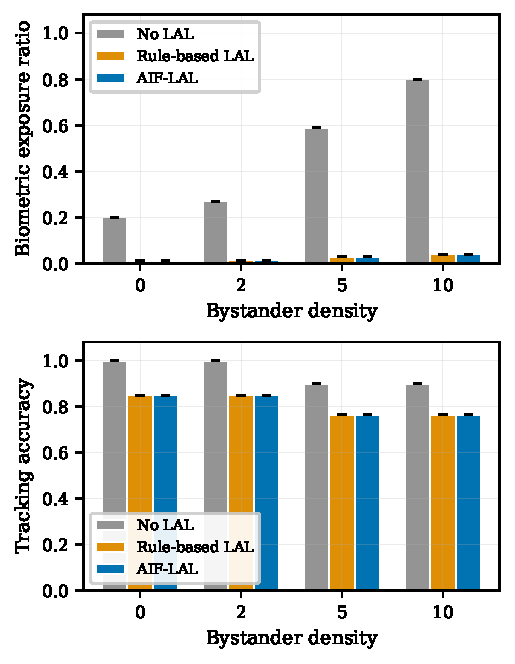
\includegraphics[width=\columnwidth]{fig1_minimization.pdf}
\caption{Biometric-exposure violation rate~(a) and tracking accuracy~(b) across three conditions and four bystander densities. The rule-based LAL pays a constant tracking penalty from blanket anonymization; the AIF-LAL, unable to rule bystanders out under the $70\%$-accurate scene cue, converges on the same anonymize-always policy and matches its exposure and tracking exactly. Error bars: $\pm 1$ s.d.\ across 100 trials.}
\label{fig:minimization}
\end{figure}


We compare three conditions across 100 trials of 20 timesteps at four bystander densities $\{0, 2, 5, 10\}$: a baseline (always RAW), a rule-based LAL (always ANONYMIZED), and the AIF-LAL (agent chooses via EFE minimization over the mixed C). Results are in Figure~\ref{fig:minimization}. The baseline leaks bystander biometrics at rates proportional to density. The rule-based LAL eliminates exposure but pays a constant tracking penalty of $\sim15\%$ relative to the baseline at every density, because blanket anonymization degrades tracking whether or not bystanders are present. The AIF agent mixes the C-profiles according to its scene posterior. Under the $70\%$-accurate scene cue that posterior never becomes confident enough that the target is alone to justify RAW capture, so the mixture keeps the pipeline anonymized throughout: exposure ($0.01$--$0.04$ across densities) and tracking accuracy ($0.85$ at $d{\leq}2$, $0.77$ at $d{\geq}5$) match the rule-based LAL exactly. The agent reproduces the hand-coded rule here rather than beating it. The equivalence still says something about the mechanism. When the agent is unsure which scene it is in, the mixture of profiles is dominated by the more cautious ones, so uncertainty about the scene pushes toward anonymizing; this is the same property that produces refusal under sensor noise in Section~\ref{sec:noise}. Selective RAW capture would require a scene sensor precise enough to establish that the target is alone. The framework makes that dependence on sensor precision explicit, where a hand-tuned rule would leave it implicit.



\subsection{Geofence Compliance (EASA)}

The agent controls its zone (SAFE, BOUNDARY, RESTRICTED, or EMERGENCY\_ZONE via STAY/ADVANCE/RETREAT). The target drifts toward restricted airspace and airspace status switches from OPEN to RESTRICTED at $t = 15$; observations are GPS zone, target bearing, a geofence alert, tracking status, and a noisy emergency-dispatch signal. Two scenarios share this schedule. In the \textit{normal} scenario urgency stays NORMAL and any presence in restricted airspace after the switch is a violation. In the \textit{emergency} scenario an override is authorized at $t = 20$: the incursion that was a violation at $t = 19$ becomes the legally correct response one step later, and the agent only learns of the switch through the dispatch channel (accuracy $0.875$). Four preference profiles are indexed by (airspace, urgency): under (RESTRICTED, NORMAL) the zone preference $C_0 = [2, 0, -4, -6]$ encodes the geofence, while under (RESTRICTED, EMERGENCY) it becomes $[0, 2, 3, -2]$, an authorized pull into restricted airspace (Appendix~\ref{app:profiles} lists all four). We compare four controllers per scenario, 50 trials each: PID-only, a rigid geofence rule, the same rule with a hard-coded exception that trusts the raw dispatch signal, and the AIF-LAL.

\begin{figure}[H]
\centering
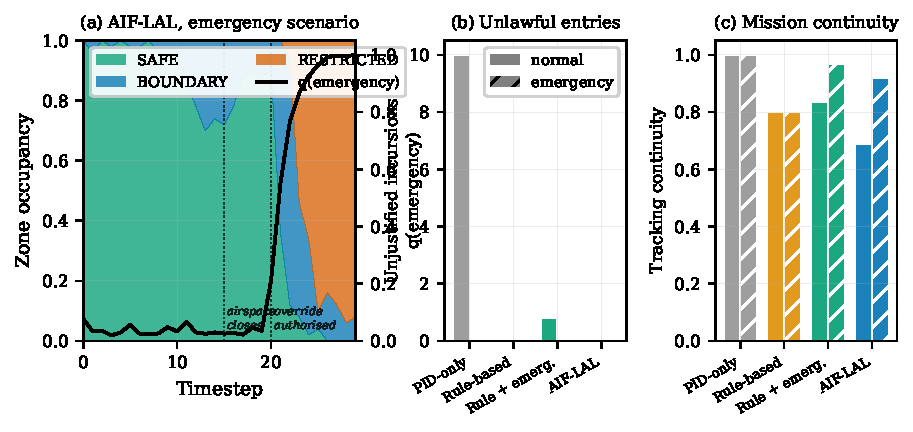
\includegraphics[width=\columnwidth]{fig2_geofence.pdf}
\caption{Geofence compliance with an emergency exception. (a)~AIF zone occupancy in the emergency scenario against the agent's belief that an override is authorized: it enters restricted airspace as $q(\text{emergency})$ resolves after the $t{=}20$ authorization. (b)~Unjustified incursions per controller and scenario. (c)~Tracking continuity. The rule with a hard-coded exception fires on dispatch noise in $0.56$ of normal trials; AIF commits no unjustified incursion in either scenario.}
\label{fig:geofence}
\end{figure}

Figure~\ref{fig:geofence} shows the results. The PID-only controller follows the target wherever it goes: perfect tracking ($1.00$), ten incursion-steps per trial, all of them unjustified in the normal scenario. The rigid rule never enters restricted airspace in either scenario, which makes it compliant in the normal case ($0.80$ tracking, zero incursions) and useless in the emergency: its override rate is $0.00$, so the authorized response never happens. Adding a hard-coded exception that trusts the raw dispatch signal repairs the emergency case ($1.00$ override rate, $0.97$ tracking) but breaks the normal one: dispatch noise triggers unjustified incursions in $0.56$ of normal trials. The AIF agent is the only controller correct in both scenarios: zero unjustified incursions in both, a $1.00$ override rate once the authorization arrives (it accumulates dispatch evidence for a few steps before committing, $5.7$ incursion-steps against the exception rule's $8.0$), and $0.92$ tracking during the emergency. The price is conservatism before context resolves: in the normal scenario it keeps more distance from the boundary than the rigid rule ($0.69$ tracking against $0.80$), it loses some tracking contact in exchange for a margin against being wrong about the airspace status, consistent with its behavior under noise (Section~\ref{sec:noise}).




\subsection{Emergency Override}

This experiment tests the central claim of the paper: that preference magnitudes can implement defeasible legal reasoning. The drone moves through four positions (PATROL, APPROACH, PRIVACY\_ZONE, TARGET) and can HOLD or ADVANCE. Privacy context (ACTIVE or SUSPENDED) and urgency (NORMAL or EMERGENCY) vary outside its control. The agent observes its own position, a privacy cue (precise near the privacy zone, ambiguous elsewhere), a noisy emergency signal, and a complaint signal that fires when it enters the privacy zone while privacy is ACTIVE.

\begin{table}[H]
\centering
\scriptsize
\resizebox{\columnwidth}{!}{%
\begin{tabular}{clll}
\toprule
\textbf{\#} & \textbf{Privacy} & \textbf{Urgency} & \textbf{Expected behavior} \\ \midrule
C1 & All ACTIVE    & All NORMAL    & Wait at approach \\
C2 & All ACTIVE    & All EMERGENCY & Cross despite complaint \\
C3 & All SUSPENDED & All NORMAL    & Cross freely \\
C4 & All SUSPENDED & All EMERGENCY & Cross immediately \\
C5 & ACTIVE$\to$SUSP & All NORMAL    & Wait, then cross \\
C6 & ACTIVE$\to$SUSP & All EMERGENCY & Cross early \\
C7 & ACTIVE$\to$SUSP & NORM$\to$EMERG & Cross when justified; timing inferred \\
\bottomrule
\end{tabular}}
\caption{Seven experimental conditions. Privacy switches at $t = 7$; urgency switches at $t = 4$. C7 is the condition we built the experiment around: emergency onset precedes privacy suspension, so the agent must decide whether to override active privacy constraints based on inferred urgency, with no known schedule to rely on.}
\label{tab:conditions}
\end{table}

Four preference profiles are indexed by (urgency, privacy). Under (NORMAL, ACTIVE) the position preference over (PATROL, APPROACH, PRIVACY\_ZONE, TARGET) is $C_0 = [0, 1, -6, -2]$ with complaint aversion $C_3 = [8, -8]$: the agent prefers to hold at APPROACH and avoids the privacy zone. Under (EMERGENCY, ACTIVE) the profile becomes $C_0 = [0, 0, 0, 6]$ with complaint aversion relaxed to $[1, -1]$. The effective preference at each timestep is the belief-weighted mixture of the four profiles, so as $q(\text{emergency})$ rises, $C_{\text{eff}}$ moves continuously from the first profile toward the second and the EFE balance tips toward advancing despite the complaint signal. Table~\ref{tab:conditions} lists seven conditions that vary privacy and urgency schedules across $T = 15$ timesteps (planning depth $N = 4$, 50 trials each). The horizon is set by the event schedule: the episode must outlive the last scheduled switch ($t = 7$) by the number of steps the agent needs to become confident that the switch has happened (the belief-integration lag) plus the steps it needs to travel to the target. An earlier version of this battery used $T = 10$, which censors exactly the post-switch behavior the delayed-switch conditions are designed to measure (see Discussion). Throughout, \textit{violation} counts entry into the privacy zone while privacy is ACTIVE, whether or not an emergency justifies the entry; on the emergency-mandated conditions a high count is the intended outcome, and we report the raw count so both readings are available.

Figure~\ref{fig:summary} summarizes all seven conditions. The agent violates privacy most often in emergency conditions (C2, C4, C6, C7), which are exactly the conditions where crossing the privacy zone is legally justified. It reaches the target whenever either privacy is suspended or emergency context provides legal grounds to override.

Figure~\ref{fig:emergency} shows representative (modal) trajectories for three conditions. Under C1 (normal urgency, active privacy), the agent reaches APPROACH and halts there: complaint aversion outweighs the mild target preference and the agent never enters the privacy zone (aggregate C1 violation rate is $0.10$, $95\%$ CI $[0.02, 0.20]$; Appendix~\ref{app:results} tabulates CIs for all conditions).

\begin{figure}[H]
\centering
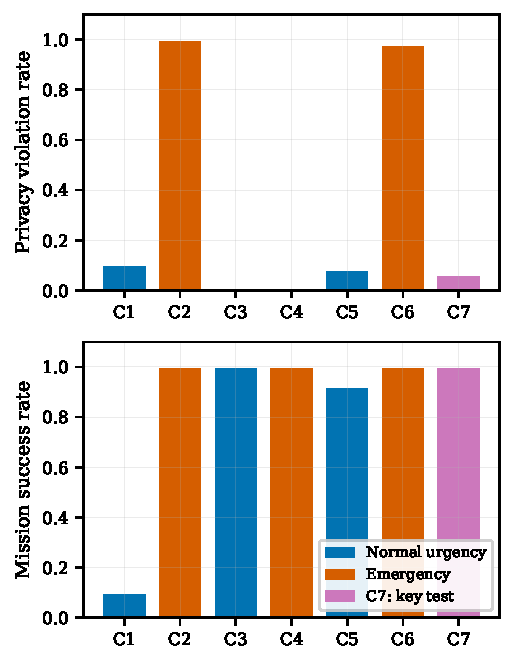
\includegraphics[width=\columnwidth]{fig4_summary.pdf}
\caption{Summary across all seven conditions. (a)~Privacy violation rate: highest under emergency conditions, where crossing is legally justified. (b)~Mission success rate: the agent reaches the target when privacy is suspended or emergency context permits override. Purple: C7.}
\label{fig:summary}
\end{figure}


Under C2 (emergency, active privacy), the agent waits at APPROACH while it builds confidence in the emergency observation, then advances through the privacy zone and reaches the target around $t{=}7$ (aggregate C2 success $1.00$, violation $1.00$ because the emergency mandates the crossing). 
 
\begin{figure*}[tp]
\centering
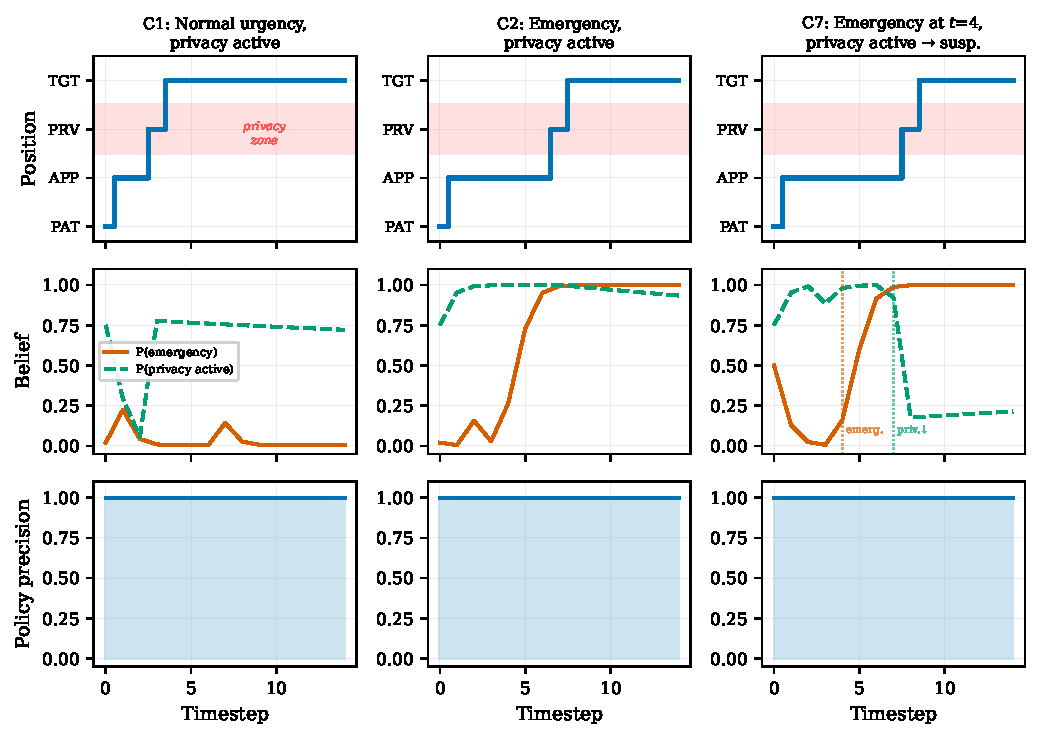
\includegraphics[width=\textwidth]{fig3_emergency.pdf}
\caption{Emergency override trajectories for C1 (normal), C2 (emergency), and C7 (emergency onset before privacy suspension). Top: drone position (privacy zone in red). Middle: inferred beliefs about emergency (solid red) and privacy active (dashed green); in C7, dotted lines mark emergency onset ($t=4$) and privacy suspension ($t=7$). Bottom: $C_{\text{eff}}$ tracking error, the $L^2$ distance between the mixed effective preference profile and the oracle profile for the true context. C1 converges quickly to the (normal, active) profile; C2 stays high because the urgency observation is noisy and the agent only commits after several timesteps; C7 shows a bimodal pattern, with error spiking at $t{=}4$ when urgency switches and falling again as the agent locks onto the new context.}
\label{fig:emergency}
\end{figure*}
 
 In C7, the agent waits at APPROACH until $t{=}7$, the timestep at which privacy switches from active to suspended, and crosses immediately after: it reaches the target on every trial, and only $6\%$ of trials cross while privacy is still active. The belief trajectories in the middle row of Figure~\ref{fig:emergency} confirm that $q(\text{emergency})$ rises around $t{=}4$ (when urgency switches) and $q(\text{privacy active})$ falls around $t{=}7$ (when privacy suspends). The same agent, with the same model and the same set of policies, produces all three behaviors; only the effective preference differs between conditions.

\subsection{Computational Overhead}

We measure wall-clock time per decision cycle over 1000 post-warmup iterations under two execution modes (Figure~\ref{fig:overhead}). PID control and audit logging are negligible in both ($0.0003\,$ms and $0.10\,$ms respectively). The two AIF numbers differ by three orders of magnitude. Running the inference--planning--sampling cycle through a Python loop with per-step JAX dispatch takes $1148 \pm 518\,$ms per cycle, dominated by Python$\,\to\,$JAX boundary overhead; the computation itself is small: the POMDP has 3 state factors of 4, 2, 2 states and a policy depth of $N{=}4$, a FLOP count that fits in a single GPU kernel launch. Wrapping the same cycle in a JIT-compiled function that processes 10 timesteps per call drops the cost to $0.31 \pm 0.08\,$ms per step ($3.07 \pm 0.77\,$ms per 10-step call, $3{,}260$ Hz throughput on an RTX 5070). The compiled cost is $3{,}700\times$ lower than the uncompiled one and well below the $100\,$ms target for direct closed-loop drone control. The $0.31\,$ms figure is steady-state per-step execution of an already-compiled scan. It is timed with \texttt{block\_until\_ready()} on each call, which forces the host to wait for the device computation to finish before the timer stops, so the value reflects completed compute on the GPU. Compilation is a separate one-time cost, reported in the next paragraph, and is excluded from this per-step number.

There are caveats. The compiled variant assumes the same observation interface for $K$ steps ahead; if the LAL receives genuinely irregular input from the perception layer it must recompile, and the JIT cost ($\sim2\,$s on first call) is paid once per code path. We also have not run on edge hardware such as the NVIDIA Jetson, where memory bandwidth and kernel launch overhead differ from a desktop GPU. Architecturally the LAL is a \textit{supervisory} layer over a faster inner controller: PID control runs at full rate while the LAL reviews actuation decisions, with the relevant cadence set by how fast legal context can change. At $0.31\,$ms per step, the compiled measurement clears even the inner-loop budget by orders of magnitude.

\begin{figure}[H]
\centering
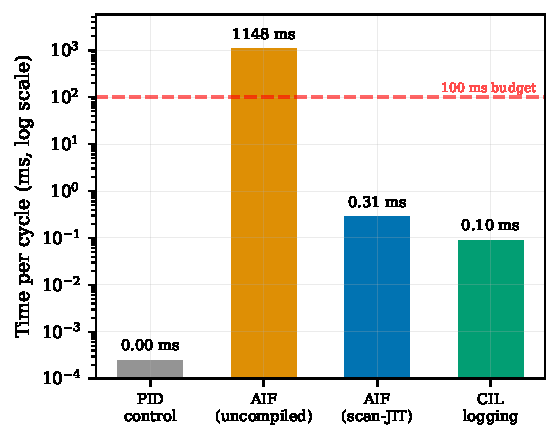
\includegraphics[width=\columnwidth]{fig5_overhead.pdf}
\caption{Per-component overhead per decision cycle (log scale). The Python-loop AIF measurement ($1148\,$ms) is dominated by per-step JAX dispatch overhead and sits an order of magnitude above the $100\,$ms target. JIT-compiling the inference--planning--sampling cycle through a 10-step scan drops the effective per-step cost to $0.31\,$ms, three orders of magnitude lower and well below the budget. PID control ($0.0003\,$ms) and CIL audit logging ($0.10\,$ms) are negligible in both modes. Measurements on an RTX 5070; we have not yet measured on edge hardware.}
\label{fig:overhead}
\end{figure}



\subsection{EFE Component Ablation}
\label{sec:ablation}

The expected free energy (Equation~\ref{eq:efe}) combines a pragmatic term (preference satisfaction) and an epistemic term (information gain about hidden states). To see which term drives the compliance behavior, we ablate the EFE by isolating each term and comparing to the full agent and to a random-action control. Each configuration uses $100$ trials on conditions C1 (normal urgency, active privacy), C5 (privacy switch, normal urgency), and C7 (the emergency-onset-before-privacy-suspension condition).

\textsc{pragmatic\_only} is statistically indistinguishable from \textsc{full} on C1 and C5 (violation $0.10$ vs.~$0.10$ and $0.08$ vs.~$0.07$; Mann--Whitney $p > 0.9$ on both): preference-driven policy selection produces the compliance behavior. On C7 the full agent violates less: both reach the target on every trial, but removing the epistemic term raises the violation rate from $0.08$ to $0.13$ ($p = 0.035$, $d = 0.21$). Information-seeking therefore adds restraint on the one condition where the timing of the context switch matters. \textsc{epistemic\_only} fails completely (success $0.00$, violation $1.00$ on all three conditions): without preferences, the agent treats the privacy zone as a high-information region and lingers there, accumulating violations while it gathers evidence about the hidden state. The epistemic term does not produce compliant behavior on its own. In the full agent it acts as a regularizer, discouraging commitment to an action before the legal context that would justify it has been inferred.

The small cost of removing it on C1 and C5 has a mechanistic explanation. Part of the caution the epistemic term would supply is already built into the mixture: while the posterior over context is unresolved, $C_{\text{eff}}$ is a blend of profiles, and a blend of a permissive and a prohibitive profile is itself cautious. The epistemic term adds something beyond this only where the informativeness of an observation depends on where the agent is. In this model that is true of one channel: the privacy cue is informative only near the zone. Moving to APPROACH to read it costs the agent almost nothing, so it happens with or without an explicit information-gain incentive, and removing the term changes little. C7 is the exception because it is the condition where the violations the term prevents are concentrated, so waiting to sense before committing pays there. Figure~\ref{fig:ablation} shows the same data plus the time the agent spends at APPROACH before advancing: \textsc{full} and \textsc{pragmatic} both wait ${\sim}6.6$--$6.8$ timesteps before committing on C7; \textsc{epistemic} commits in $1$ timestep (straight into the privacy zone for information gain); \textsc{random} averages $\sim 2$.

\begin{figure}[H]
\centering
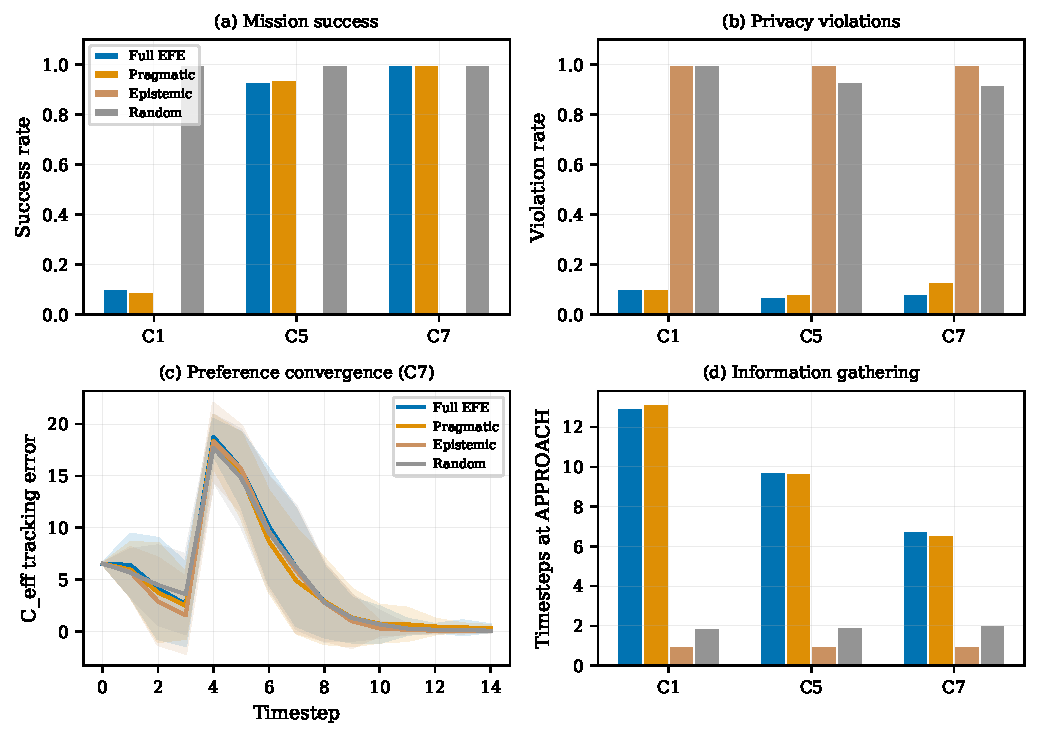
\includegraphics[width=\columnwidth]{fig6_ablation.pdf}
\caption{EFE ablation across C1, C5, C7 (100 trials/cell, $T{=}15$, $N{=}4$). (a) Success and (b) violation rates by EFE configuration. (c)~C\textsubscript{eff} tracking error over time for C7. (d)~Timesteps spent at APPROACH before advancing. Epistemic-only fails because information gain without preferences drives the agent into the privacy zone for evidence.}
\label{fig:ablation}
\end{figure}


\subsection{Comparison Against Baseline Agents}
\label{sec:baselines}

We compare the AIF-LAL against three baseline agents on all seven conditions, $100$ trials each. \textsc{hpm\_oracle} is a Hierarchical Predictive Model: a two-level prediction-error minimizing controller (low level: motor command, high level: legal context) that decides whether to cross by thresholding the high-level posterior. The oracle variant is given the true urgency and privacy state at each timestep. \textsc{hpm\_noisy} uses the same architecture but receives noisy context. \textsc{bayes\_rules} is a Bayesian state estimator wired to a deterministic if-then rule on the single most-likely (maximum-a-posteriori) hidden state. Table~\ref{tab:baselines} reports success/violation per condition.

\begin{table}[H]
\centering
\scriptsize
\resizebox{\columnwidth}{!}{%
\begin{tabular}{lccccccc}
\toprule
\textbf{Agent} & C1 & C2 & C3 & C4 & C5 & C6 & C7 \\ \midrule
AIF          & .12/.13 & 1/1 & 1/0 & 1/0 & .93/.13 & 1/.97 & 1/.19 \\
HPM\_ORACLE  & 0/0     & 1/1 & 1/0 & 1/0 & 1/0     & 1/1   & 1/1 \\
HPM\_NOISY   & .83/.98 & 1/1 & 1/0 & 1/0 & 1/.78   & 1/1   & 1/1 \\
BAYES\_RULES & .09/.31 & 1/1 & 1/0 & 1/0 & 1/.24   & 1/.99 & 1/.79 \\ \bottomrule
\end{tabular}}
\caption{Baseline comparison: success/violation per condition, $n{=}100$ trials. On C7 (emergency onset before privacy suspension), AIF is the only agent that keeps privacy violations low, at full mission completion; the three baselines all violate at $0.79$--$1.00$ on C7. \textsc{hpm\_oracle} matches the desired pattern on C5 (where the agent should wait until privacy suspends, then cross) but not on C7, because its rule does not condition on \textit{when} the emergency was authorized. AIF rates differ from Section~5.3's aggregates (e.g.,~C1 $.13$ vs $.10$, C7 violation $.19$ vs $.06$): each experiment is an independent run with its own seeds and trial count; per-condition confidence intervals are in Appendix~\ref{app:results}.}
\label{tab:baselines}
\end{table}

The C7 numbers are where the agents differ. \textsc{hpm\_oracle}, even given the true context, reaches the target $1.00$ of the time and violates privacy $1.00$ of the time: a rule that knows the context still crosses while privacy is active, because it does not condition on \textit{when} the emergency authorization arrived. \textsc{hpm\_noisy} and \textsc{bayes\_rules} both violate at $0.79$--$1.00$ on C7. AIF reaches the target on every trial with $0.19$ violation, a combination none of the baselines reach. On C5 (privacy suspends at $t{=}7$, no emergency), \textsc{hpm\_oracle} still has the edge: it achieves $1.0$ success / $0$ violation by waiting until $t{=}7$ and crossing then, while AIF's belief-driven timing is imperfect ($0.93$ success, $0.13$ violation). AIF is therefore not the best agent on every condition. It is the only correct one on C7, the condition where the legal trigger (emergency at $t{=}4$) and the privacy constraint (active until $t{=}7$) are out of phase.

The C7 separation does not depend on tuning. During $t = 4$--$6$, C7 presents the same context as C2: an emergency is under way and privacy is still active. A rule that maps the current context to an action, with no memory of how long that context has held, must therefore do the same thing in both conditions. If it crosses, it violates C7's still-active constraint early; if it refuses, it fails C2's mandated override. Telling the two apart requires integrating evidence over time, which is what the belief-weighted mixture does. In C2 the agent has accumulated enough confidence in the emergency to cross by $t \approx 7$. In C7 the three timesteps of emergency evidence available before $t = 7$ have not yet shifted $C_{\text{eff}}$ far enough to cross, privacy then suspends, and only a minority of trials cross earlier ($0.06$ in the Section~5.3 battery, $0.19$ under this experiment's seeds). Belief-weighted profile mixing also produces graded behavior across the four context combinations (Figure~\ref{fig:baselines}).

\begin{figure}[H]
\centering
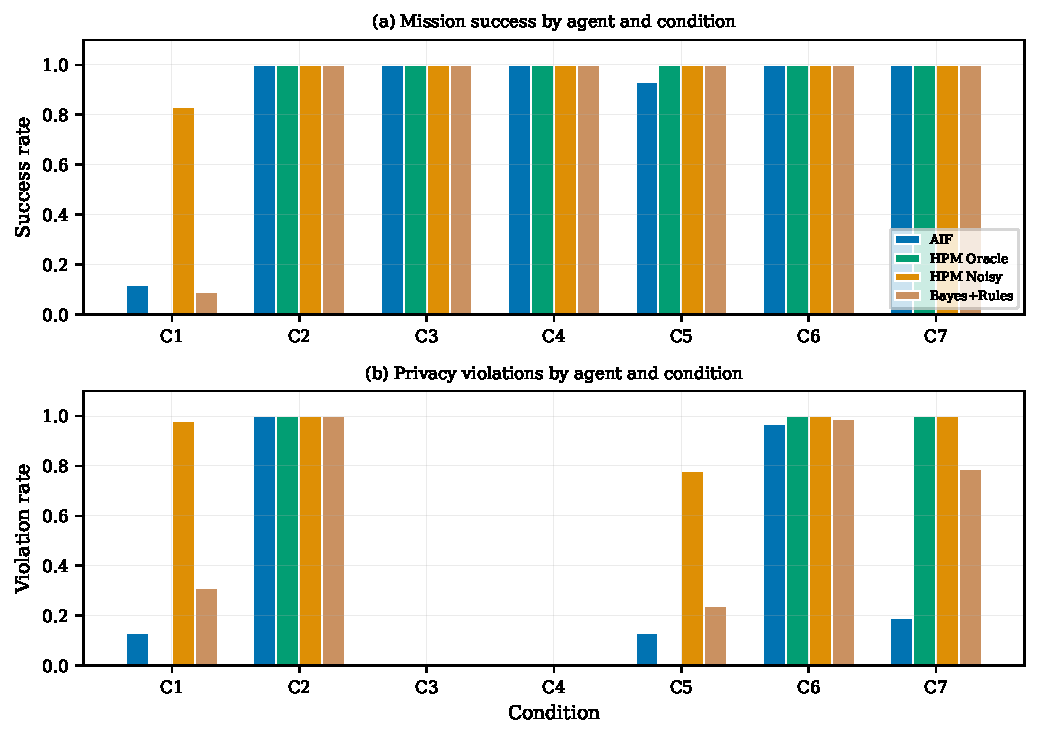
\includegraphics[width=\columnwidth]{fig7_baselines.pdf}
\caption{Baseline comparison across C1--C7. On C7 (emergency at $t{=}4$, privacy lifts at $t{=}7$), AIF-LAL (blue) is the only agent that combines high success with low violation; all three baselines violate at $0.79$--$1.00$. On the simpler privacy-active conditions C1 and C5, \textsc{hpm\_oracle} (with the true context) matches or beats AIF.}
\label{fig:baselines}
\end{figure}


\subsection{Sensitivity to Preference Magnitudes}
\label{sec:sensitivity}

We sweep the two preference magnitudes that most directly govern emergency override: the emergency target drive (ETD, the value of $C_0[3]$ under EMERGENCY context, swept over $\{0.5, 1, 2, 3, 4, 6, 8\}$) and the normal complaint aversion (NCA, the value of $C_3[1]$ under NORMAL context, swept over $\{2, 4, 6, 8, 10\}$). For each $(ETD, NCA)$ cell we run $50$ trials of the seven-condition test and report the \textit{override score} $P(\text{cross} \mid \text{emergency}) - P(\text{cross} \mid \text{normal})$. A high score means the agent crosses under emergency and refrains under normal context, which is the intended behavior.

The surface has a broad ridge along $\text{ETD}{\in}[1,3]$, $\text{NCA}{\in}[4,10]$, peaking at $0.86$ at $(\text{ETD}, \text{NCA}) = (1, 6)$ and $(1, 8)$. The sweep uses a simplified two-parameter profile family rather than the full headline profiles; in its coordinates, the headline values of Section~5.3 correspond to $(\text{ETD}, \text{NCA}) = (6, 8)$, which scores $0.72$: on the ridge, but not at its peak. We did not tune the headline experiments to the sweep optimum.

\begin{table}[H]
\centering
\scriptsize
\begin{tabular}{c|ccccc}
\toprule
\textbf{ETD\textbackslash NCA} & 2 & 4 & 6 & 8 & 10 \\ \midrule
0.5 & 0.08 & 0.10 & 0.16 & 0.12 & 0.10 \\
1.0 & 0.58 & 0.70 & \textbf{0.86} & \textbf{0.86} & 0.78 \\
2.0 & 0.48 & 0.68 & 0.80 & 0.76 & 0.78 \\
3.0 & 0.44 & 0.60 & 0.76 & 0.80 & 0.84 \\
4.0 & 0.60 & 0.64 & 0.68 & 0.76 & 0.70 \\
6.0 & 0.50 & 0.52 & 0.64 & 0.72 & 0.72 \\
8.0 & 0.18 & 0.46 & 0.58 & 0.70 & 0.64 \\ \bottomrule
\end{tabular}
\caption{Override score $P(\text{cross}|\text{emergency}) - P(\text{cross}|\text{normal})$ over a $7{\times}5$ ETD/NCA sweep at $T = 15$. Maximum at $\text{ETD}{=}1$, $\text{NCA}{\in}\{6, 8\}$. The score declines gradually at very high ETD or very low NCA.}
\label{tab:sensitivity}
\end{table}

At very low ETD ($0.5$) the emergency context cannot pull the agent across and the score collapses; at very high ETD ($8$) with low NCA ($2$) the emergency drive leaks into the normal condition, $P(\text{cross}|\text{normal})$ rises, and the score erodes to $0.18$. Both failure modes are gradual: the framework tolerates roughly an order of magnitude of misspecification on each axis before behavior degrades (Figure~\ref{fig:sensitivity}).

\begin{figure}[H]
\centering
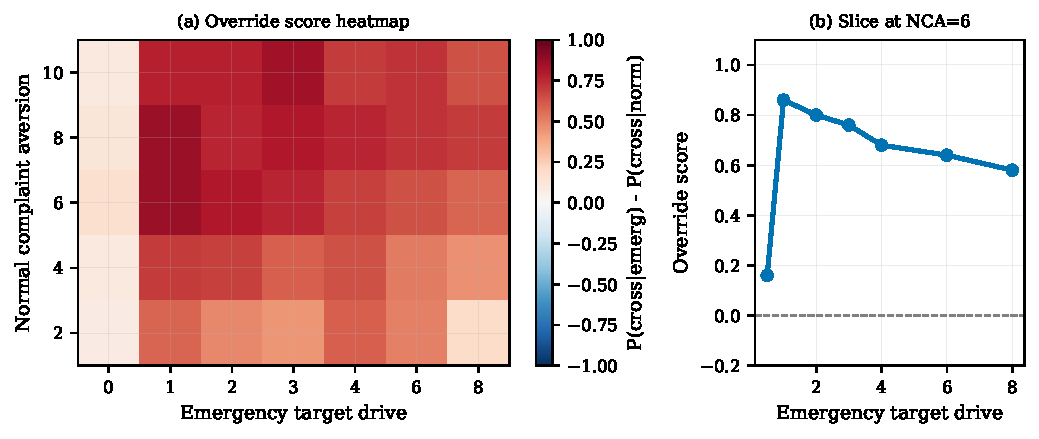
\includegraphics[width=\columnwidth]{fig8_sensitivity.pdf}
\caption{Sensitivity sweep: override score over the $(\text{ETD}, \text{NCA})$ grid. A broad ridge of high scores shows that the framework tolerates moderate misspecification of preference magnitudes; the headline values sit on this ridge (see text).}
\label{fig:sensitivity}
\end{figure}


\subsection{Robustness to Observation Noise}
\label{sec:noise}

Real sensors are noisy. We perturb the $\mathbf{A}$ matrices with Dirichlet noise of increasing concentration ($\nu \in \{0.01, 0.05, 0.125, 0.2, 0.3, 0.4, 0.49\}$) and rerun three agents (AIF, \textsc{hpm\_noisy}, \textsc{bayes\_rules}) on C1 and C7, $100$ trials each. Table~\ref{tab:noise} reports C7 results. Belief-weighted profile mixing has a useful failure mode under high noise. The agent's posterior over privacy and urgency becomes less peaked, the mixed $C_{\text{eff}}$ blends toward conservative profiles, and the policy stops committing to actions that depend on confident context. 


\begin{table}[H]
\centering
\scriptsize
\resizebox{\columnwidth}{!}{%
\begin{tabular}{lccc}
\toprule
\textbf{Noise} & \textbf{AIF C7 s/v} & \textbf{HPM\_NOISY C7 s/v} & \textbf{BAYES\_RULES C7 s/v} \\ \midrule
0.01  & 1.00/1.00 & 1.00/1.00 & 1.00/1.00 \\
0.05  & 1.00/\textbf{0.14} & 1.00/1.00 & 1.00/0.93 \\
0.125 & 1.00/\textbf{0.11} & 1.00/1.00 & 1.00/0.85 \\
0.20  & 0.99/\textbf{0.11} & 1.00/1.00 & 1.00/0.47 \\
0.30  & 0.91/\textbf{0.21} & 1.00/1.00 & 0.91/0.33 \\
0.40  & 0.73/\textbf{0.11} & 1.00/0.99 & 0.66/0.15 \\
0.49  & 0.20/\textbf{0.00} & 1.00/1.00 & 0.00/0.00 \\ \bottomrule
\end{tabular}}
\caption{Noise sweep on C7. At near-zero noise every agent crosses at emergency onset; from $\nu = 0.05$ on, AIF holds violation at $0.11$--$0.21$ while sustaining success $0.73$--$1.00$ through $\nu = 0.4$. \textsc{hpm\_noisy} violates at ${\sim}1.00$ throughout; \textsc{bayes\_rules} degrades toward inaction with higher violations along the way. At extreme noise ($0.49$) AIF mostly stops acting ($0.20$ success, $0.00$ violations); \textsc{hpm\_noisy} continues to cross indiscriminately.}
\label{tab:noise}
\end{table}


\begin{figure}[tp]
\centering
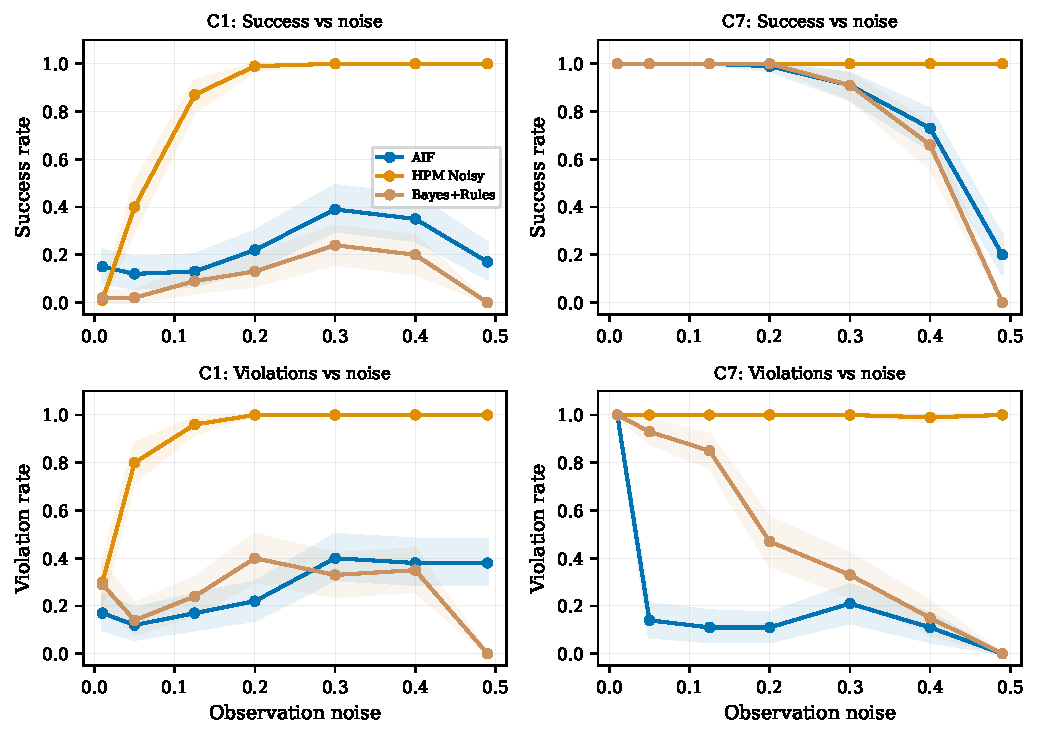
\includegraphics[width=\columnwidth]{fig9_noise.pdf}
\caption{Noise robustness on C1 and C7 across seven noise levels. On C7, AIF holds violations at ${\leq}0.21$ for $\nu \in [0.05, 0.4]$ where \textsc{hpm\_noisy} stays near $1.00$; on C1, AIF violations rise with noise (to $0.40$ at $\nu{=}0.3$) as context inference degrades. The trade-off is reduced success at very high noise, but the missed successes coincide with violations the baselines would have committed.}
\label{fig:noise}
\end{figure}

Baselines that threshold to the single most-likely hidden state instead compound observation errors into policy errors. At $\nu = 0.49$ (near-uninformative observations) AIF largely stops acting ($0.20$ success with $0.00$ violations) and \textsc{bayes\_rules} stops entirely ($0.00/0.00$); \textsc{hpm\_noisy} continues to cross with violation $1.00$. AIF's success rate on C7 declines gracefully ($0.91$ at $\nu{=}0.3$, $0.73$ at $\nu{=}0.4$, $0.20$ at $\nu{=}0.49$), and the trials it gives up are the trials on which the baselines violate (Figure~\ref{fig:noise}).




\subsection{Model Acquisition and the Calibrated-Sensor Principle}
\label{sec:learning}


\begin{figure*}[tp]
\centering
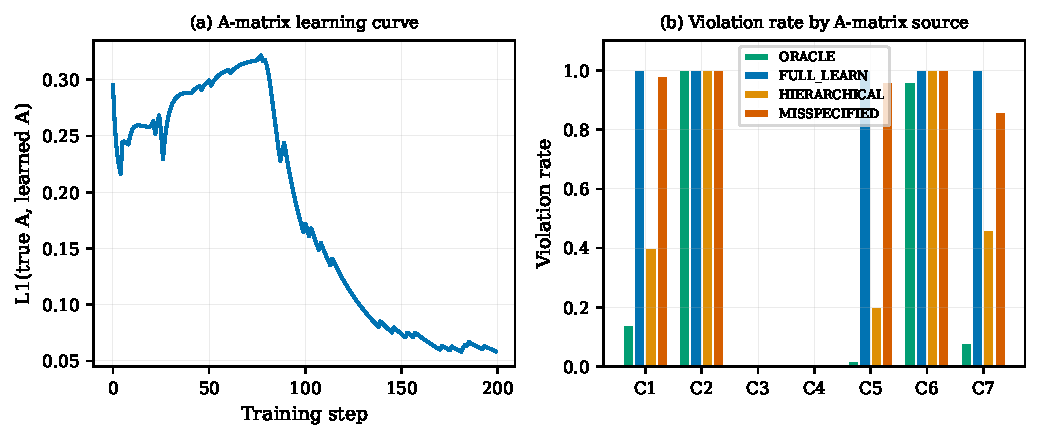
\includegraphics[width=\textwidth]{fig10_learning.pdf}
\caption{(a) $L^1$ distance between learned and true $A_2$ during flat-prior training. (b) Violation rate across configurations on C1--C7. \textsc{full\_learn} collapses to maximum violation on the privacy-active conditions; \textsc{hierarchical} recovers full success and half or more of the lost compliance; the residual C1/C7 gap is left by the unlearned sanction channel.}
\label{fig:learning}
\end{figure*}

All preceding experiments assume the agent is given the true observation model $\mathbf{A}$. We now ask whether $\mathbf{A}$ can instead be \textit{learned} from experience. We train the agent for $200$ environment steps with weakly informative Dirichlet priors on every modality, then freeze the learned $\mathbf{A}$ and test it on the seven-condition battery. We compare four configurations: \textsc{oracle} (true $\mathbf{A}$), \textsc{full\_learn} (all four modalities learned from uniform priors), \textsc{hierarchical} (modalities $A_0$ position and $A_2$ emergency signal fixed by construction with strong Dirichlet concentration $\alpha{=}10^4$ on their true values; modalities $A_1$ privacy cue and $A_3$ complaint learned from uniform priors), and \textsc{misspecified} (true $\mathbf{A}$ with the $A_1$ privacy cue polarity inverted; provides an upper bound on the cost of getting $A_1$ wrong).

\begin{table}[H]
\centering
\scriptsize
\resizebox{\columnwidth}{!}{%
\begin{tabular}{lccccccc}
\toprule
\textbf{Config} & C1 & C2 & C3 & C4 & C5 & C6 & C7 \\ \midrule
ORACLE        & .12/.14 & 1/1 & 1/0   & 1/0 & .96/.02 & 1/.96 & 1/.08 \\
FULL\_LEARN   & 1/1     & 1/1 & 1/0   & 1/0 & 1/1     & 1/1   & 1/1 \\
HIERARCHICAL  & .38/.40 & 1/1 & 1/0   & 1/0 & 1/.20   & 1/1   & 1/.46 \\
MISSPECIFIED  & .98/.98 & 1/1 & .12/0 & 1/0 & 1/.96   & 1/1   & 1/.86 \\ \bottomrule
\end{tabular}}
\caption{Learning configurations on C1--C7, $50$ trials each. \textsc{full\_learn} collapses to maximum violation on every privacy-active condition: na\"ive learning destroys the discrimination needed for emergency override. \textsc{hierarchical} recovers full mission success and half or more of the lost compliance; the residual gap to \textsc{oracle} traces to the sanction channel, which a compliant agent cannot learn from data (see text).}
\label{tab:learning}
\end{table}

\textsc{full\_learn} produces $1.00/1.00$ on every privacy-active condition (C1, C5, C7), behavior indistinguishable from \textsc{misspecified}. This is not because the learned model is far from the truth in aggregate. After training, the learned emergency-signal matrix sits within $L^1 = 0.06$ of the truth, and C7 violation is nonetheless $1.00$. A small error in norm is enough to reverse the behavior.

The mechanism is in the EFE planner. The pragmatic-value term computes a predicted distribution over future observations under each candidate policy using $\mathbf{A}$. When $\mathbf{A}$ is imperfect, the policy that maximizes apparent preference satisfaction is no longer the policy that satisfies the actual preferences: the preference encoding is unchanged, but the planner that rolls it forward through the learned likelihood is corrupted.

\textsc{hierarchical} repairs part of the planner by keeping two observation channels at their calibrated values: position ($A_0$, the GPS analog) and the emergency dispatch signal ($A_2$). The remaining channels (privacy cue, complaint) are still learned from uniform priors. Mission success returns to $1.00$ everywhere and violations drop from $1.00$ to $0.20$ (C5), $0.40$ (C1), and $0.46$ (C7); the emergency-mandated conditions (C2, C4, C6) are unaffected. That is half or more of the lost compliance recovered, but it is well short of \textsc{oracle}'s $0.02$--$0.14$, and the training trace shows why. In $200$ training steps the compliant agent enters the privacy zone exactly once, so the complaint channel, the only sanction signal in the model, retains almost no discriminability: the learned $A_3$ predicts a complaint in the zone at $0.64$ under active privacy versus $0.54$ under suspended, against the true $0.875$ versus $0.125$. When the complaint model cannot tell the two contexts apart, the agent expects roughly the same complaint whether or not privacy is active, so the $[8, -8]$ complaint aversion no longer discourages crossing specifically when privacy is active; it becomes a near-constant offset. The learned privacy cue is degraded the same way (at APPROACH it reads active-like under both contexts, $0.93$ versus $0.74$, against the true $0.875$ versus $0.125$), because belief-weighted updates smear observations across privacy contexts the agent never confidently resolved. More training will not close the gap, because the observations that would teach the agent the sanction channel are observations of its own violations, which a compliant agent does not produce. Figure~\ref{fig:learning} plots the full picture.


For a compliance system, the standard active-inference recipe of weak priors on every modality plus end-to-end learning is not safe. Observation channels that determine \textit{whether} an obligation applies (the GPS that says the drone has entered restricted airspace, the dispatch protocol that says an override is authorized) need to come from hardware calibration. Environmental channels can be learned, but only to the extent that a compliant policy actually samples them, and the sanction channel is the worst case, because sampling it means violating. A deterrent that must be reliable therefore needs its observation model specified in advance rather than learned.


%% ─────────────────────────────────────────────────────────
\section{Discussion}
%% ─────────────────────────────────────────────────────────
As Figure~\ref{fig:concept} summarizes, the Legal Actuator Layer compiles statute into preferences and resolves competing obligations by minimizing expected free energy.

\begin{figure*}[tp]
\centering
\resizebox{\textwidth}{!}{%
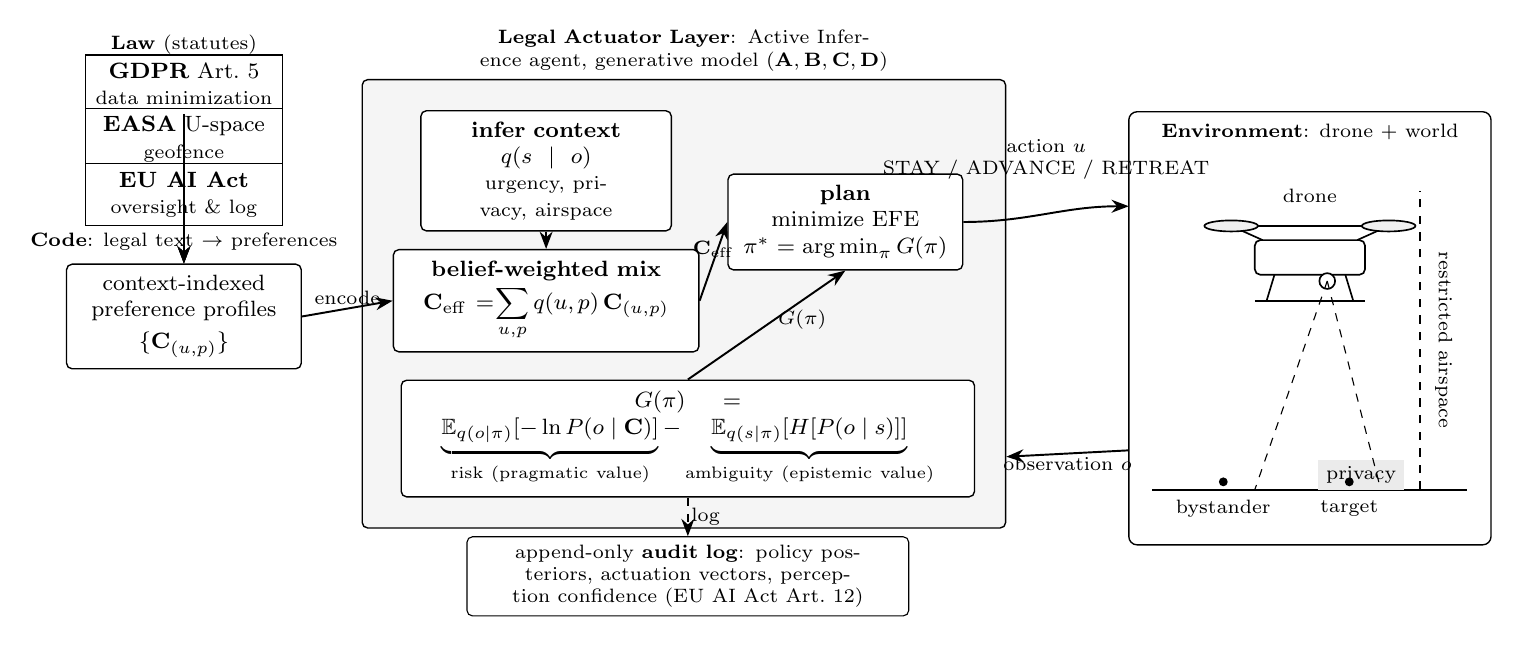
\begin{tikzpicture}[
  x=1cm,y=1cm,
  font=\footnotesize,
  >={Stealth[length=2.2mm]},
  box/.style={draw, rounded corners=2pt, align=center, inner sep=4pt, line width=0.5pt},
  sub/.style={draw, rounded corners=2pt, align=center, inner sep=4pt, fill=white, line width=0.5pt},
  doc/.style={draw, align=center, inner sep=3pt, line width=0.5pt, minimum width=2.5cm, fill=white},
  lab/.style={align=center, font=\scriptsize, inner sep=1pt},
  flow/.style={->, line width=0.7pt},
  dflow/.style={->, line width=0.6pt, dashed},
]

%% ---------- STAGE A: LAW AS CODE ----------
\node[lab] at (1.4,7.05) {\textbf{Law} (statutes)};
\node[doc] (gdpr)  at (1.4,6.55) {\textbf{GDPR} Art.~5\\\scriptsize data minimization};
\node[doc] (easa)  at (1.4,5.85) {\textbf{EASA} U-space\\\scriptsize geofence};
\node[doc] (aiact) at (1.4,5.15) {\textbf{EU AI Act}\\\scriptsize oversight \& log};
\node[lab] at (1.4,4.55) {\textbf{Code}: legal text $\rightarrow$ preferences};
\node[box, text width=2.7cm] (cprof) at (1.4,3.6)
  {context-indexed\\ preference profiles\\[2pt] $\{\mathbf{C}_{(u,p)}\}$};
\draw[flow] (gdpr.south)  -- (cprof.north);
\draw[flow] (easa.south)  -- (cprof.north);
\draw[flow] (aiact.south) -- (cprof.north);

%% ---------- STAGE B: AIF AGENT ----------
\node[sub, text width=2.9cm] (infer) at (6.0,5.45)
  {\textbf{infer context}\\ $q(s\mid o)$\\\scriptsize urgency, privacy, airspace};
\node[sub, text width=3.6cm] (mix) at (6.0,3.8)
  {\textbf{belief-weighted mix}\\[1pt] $\displaystyle \mathbf{C}_{\mathrm{eff}}=\!\!\sum_{u,p} q(u,p)\,\mathbf{C}_{(u,p)}$};
\node[sub, text width=2.7cm] (plan) at (9.8,4.8)
  {\textbf{plan}\\ minimize EFE\\ $\pi^{*}=\operatorname*{arg\,min}_{\pi} G(\pi)$};
\node[sub, text width=7.0cm] (efe) at (7.8,2.05)
  {$\displaystyle G(\pi)=\underbrace{\mathbb{E}_{q(o\mid\pi)}\!\left[-\ln P(o\mid \mathbf{C})\right]}_{\text{risk (pragmatic value)}}-\underbrace{\mathbb{E}_{q(s\mid\pi)}\!\left[H[P(o\mid s)]\right]}_{\text{ambiguity (epistemic value)}}$};
\begin{scope}[on background layer]
\node[box, fill=black!4, fit=(infer)(mix)(plan)(efe), inner sep=11pt] (agent) {};
\end{scope}
\node[lab, anchor=south, text width=8.8cm] at ($(agent.north)+(0,0.06)$)
  {\textbf{Legal Actuator Layer}: Active Inference agent, generative model $(\mathbf{A},\mathbf{B},\mathbf{C},\mathbf{D})$};
\draw[flow] (cprof.east) -- (mix.west) node[midway,above,lab]{encode};
\draw[flow] (infer.south) -- (mix.north);
\draw[flow] (mix.east) -- (plan.west) node[midway,above,lab]{$\mathbf{C}_{\mathrm{eff}}$};
\draw[flow] (efe.north) -- (plan.south) node[pos=0.55,right,lab]{$G(\pi)$};

%% ---------- STAGE C: ENVIRONMENT ----------
\draw[rounded corners=3pt, line width=0.5pt] (13.4,0.7) rectangle (18.0,6.2);
\node[lab] at (15.7,5.95) {\textbf{Environment}: drone + world};
\begin{scope}[shift={(15.7,4.35)}, line width=0.6pt]
  \draw[rounded corners=2pt] (-0.7,-0.22) rectangle (0.7,0.22);
  \draw (-1.0,0.40) -- (1.0,0.40);
  \draw (-0.6,0.22) -- (-1.0,0.40);
  \draw (0.6,0.22)  -- (1.0,0.40);
  \draw[fill=black!6] (-1.0,0.40) ellipse (0.34 and 0.07);
  \draw[fill=black!6] (1.0,0.40)  ellipse (0.34 and 0.07);
  \draw (-0.45,-0.22) -- (-0.55,-0.55);
  \draw (0.45,-0.22)  -- (0.55,-0.55);
  \draw (-0.7,-0.55)  -- (0.7,-0.55);
  \draw[fill=white] (0.22,-0.30) circle (0.10);
  \coordinate (cam) at (0.22,-0.30);
  \node[lab] at (0,0.78) {drone};
\end{scope}
\draw[line width=0.6pt] (13.7,1.4) -- (17.7,1.4);
\fill[black!8] (15.8,1.4) rectangle (16.9,1.78);
\node[lab] at (16.35,1.59) {\scriptsize privacy};
\draw[dashed,line width=0.6pt] (17.1,1.4) -- (17.1,5.2);
\node[lab,rotate=-90] at (17.4,3.3) {restricted airspace};
\fill (16.2,1.5) circle (1.6pt); \node[lab] at (16.2,1.16) {target};
\fill (14.6,1.5) circle (1.6pt); \node[lab] at (14.6,1.16) {bystander};
\draw[dashed] (cam) -- (15.0,1.4);
\draw[dashed] (cam) -- (16.6,1.4);

%% ---------- LOOP ARROWS ----------
\draw[flow] (plan.east) to[out=0,in=180] (13.4,5.0);
\node[lab,align=center] at (12.35,5.6) {action $u$\\\scriptsize STAY / ADVANCE / RETREAT};
\draw[flow] (13.4,1.9) -- ($(agent.south east)!0.16!(agent.north east)$)
   node[midway,below,lab]{observation $o$};
\node[draw, rounded corners=2pt, align=center, fill=white, inner sep=3pt,
      font=\scriptsize, text width=5.4cm] (audit) at (7.8,0.3)
   {append-only \textbf{audit log}: policy posteriors, actuation vectors, perception confidence (EU AI Act Art.~12)};
\draw[dflow] (efe.south) -- (audit.north) node[midway,right,lab]{log};
\end{tikzpicture}}
\caption{Conceptual overview of the Legal Actuator Layer. Statutes (GDPR Art.~5, EASA U-space, EU AI Act) are compiled into context-indexed preference profiles $\{\mathbf{C}_{(u,p)}\}$: this is the law-as-code step. The drone hosts an Active Inference agent with generative model $(\mathbf{A},\mathbf{B},\mathbf{C},\mathbf{D})$. The agent infers the hidden legal context $q(s\mid o)$ from observations, forms an effective preference $\mathbf{C}_{\mathrm{eff}}$ as a belief-weighted mixture of the statutory profiles, and selects the policy that minimizes expected free energy $G(\pi)$, whose risk term scores predicted outcomes against $\mathbf{C}$ and whose ambiguity term rewards information gathering before commitment. The selected action drives the drone in a world containing a privacy zone and restricted airspace; the resulting observations close the loop, and every decision is written to an append-only audit log for EU AI Act traceability.}
\label{fig:concept}
\end{figure*}


Rule-based compliance systems encode law as hard constraints: ``never enter the restricted zone,'' ``always anonymize.'' This works until obligations compete, at which point the system either violates one rule or deadlocks. Encoding obligations as preferences with magnitudes avoids this, but priority ordering through weighted preferences is not unique to Active Inference; any multi-objective optimization can implement it, and defeasible logic frameworks have done so for decades~\cite{prakken2015}. AIF adds two things that the EFE (Equation~\ref{eq:efe}) makes possible.

The more distinctive one is \textit{context inference under uncertainty}. The agent infers its legal context before acting. The ambiguity term in the EFE rewards information-gathering: in both conflict experiments, the agent accumulates evidence about urgency for several steps before committing to an incursion, where a rule fed the same sensor commits immediately, and the component ablation locates its contribution exactly where context timing matters (C7 violations rise from $0.08$ to $0.13$ without it). A symbolic defeasible-logic system requires context as a known input; an AIF agent estimates it from noisy observations. The agent reproduces the priority structure of defeasible reasoning, where context determines which obligation prevails, through fixed context-dependent preferences; it does not perform structural non-monotonic revision of its model (for example Bayesian model expansion), and the cases we test do not require it to.

The other is that conflicts resolve into graded compromise: where obligations compete, the agent settles on an intermediate course. In the geofence experiment's emergency scenario, the agent neither refuses the override (as the rigid rule does) nor fires on the raw dispatch signal (as the hard-coded exception does): it accumulates evidence for a few steps and then commits, entering restricted airspace later than the exception rule but without its unjustified incursions. This intermediate behavior falls out of the EFE optimization over the belief-weighted mixture.

The emergency override experiment exhibits both properties: a single agent with context-dependent $\mathbf{C}$ vectors handles seven distinct legal scenarios, including the case where an emergency must override active privacy constraints, without rule switching. The baseline comparison (Section~\ref{sec:baselines}) makes this concrete. Even when a rule-based hierarchical predictive model is given the true context, it still violates on C7, because the rule does not know \textit{when} the emergency justifies the override; only the AIF agent both completes the mission once the emergency permits it and keeps violations low while privacy is still active.

The component ablation (Section~\ref{sec:ablation}) shows that the pragmatic (preference) term, not the epistemic (information-gain) term, produces the compliance behavior on its own. The epistemic term still matters: when present, it discourages commitment to actions whose outcome depends on context the agent has not yet inferred. Under sensor noise (Section~\ref{sec:noise}), belief-weighted profile mixing gets more conservative on its own: a less peaked posterior over context yields a blended $C_{\text{eff}}$ that pulls toward refusal, while baselines that threshold to a single most-likely state compound observation error into policy error. This conservatism follows from the mixing rule itself: because the profiles are log-preferences, belief-weighted averaging is a geometric pool over the corresponding preference distributions, and a geometric pool penalizes any action that some plausible context strongly disfavors. In plain terms, if the agent still gives real weight to a context under which an action would be a serious violation, that action is scored down in the mixture even when the other contexts would permit it. The risk-neutral alternative, mixing preference probabilities and then taking the log, would let a moderately confident belief in SUSPENDED wash out the ACTIVE profile's complaint aversion. For a compliance layer the geometric pool is the defensible choice, and the refusal behavior under noise follows from it.

The evaluation horizon deserves the same scrutiny as the model, because a horizon artifact can look like a mechanism result. At $T = 10$ the battery ended three steps after the last scheduled context switch, and the delayed-switch conditions looked like failures: C5 success was $0.08$ and C7 $0.76$, numbers that read as the agent refusing to act. We extended the horizon to $T = 15$. The value was chosen from the event schedule, not from the results: the episode has to outlive the last switch by the steps the agent needs to become confident the switch has happened plus the steps it needs to reach the target. With no change to the model, C5 rose to $0.92$ and C7 to $1.00$. The agent had been crossing correctly all along, and the clock had simply run out on it. We also tested the alternative repair of making the transition priors less persistent so that beliefs integrate faster. That fixes C5 but roughly triples C1 violations, because a model that admits evidence faster also admits noise faster. The horizon extension carries a milder version of the same cost (C1 violations rise from $0.04$ to $0.10$), since every added step is another draw from the small per-step probability of drifting across the zone. Some trade between stability and responsiveness is unavoidable here. Setting the horizon from the event schedule at least keeps that trade out of the tuning loop.

The learning experiment (Section~\ref{sec:learning}) marks where the framework breaks. Acquiring the full observation model from weakly informative Dirichlet priors collapses compliance behavior, even when the average $L^1$ error between learned and true $\mathbf{A}$ is small. The cause is in the EFE planner: small $\mathbf{A}$ errors corrupt the pragmatic-value calculation, and the explicit preference encoding cannot compensate. Keeping the legally relevant observation channels at hardware-calibrated values and learning only the environmental channels (Section~\ref{sec:learning}) recovers full mission success and most of the lost compliance, but not all of it: the sanction channel stays near its prior because a compliant agent almost never samples the violation state that would teach it, and a sanction model that does not discriminate between contexts cannot deter. In a compliance setting, sensor calibration on the legally relevant channels, including the channels that carry sanctions, is a precondition for the behavioral guarantees the framework otherwise provides.

The approach has limitations. Legal obligations are encoded as soft preferences, so a sufficiently strong competing preference could in principle override any of them; combining AIF preference reasoning with hard safety constraints from constrained MDPs~\cite{garcia2015} is a natural extension. Under high observational ambiguity the agent already stops acting (Section~\ref{sec:noise}), so in the regimes we tested the soft-preference design does not produce confident violation when context is unresolved; the residual gap a constrained-MDP layer would close is the absence of a hard guarantee. Translating legal language into specific preference magnitudes still demands domain expertise; the sensitivity sweep (Section~\ref{sec:sensitivity}) shows the framework tolerates roughly an order of magnitude of misspecification on the two main axes, but tuning across many obligations is open. The simulations use discrete POMDPs with hand-crafted transition matrices; real deployment would need a hybrid architecture where AIF handles legal decisions and a conventional controller handles continuous kinematics. The discrete state factors used here are deliberately minimal stand-ins for the legal triggers under study (airspace status, privacy status, urgency), and are not a model of the full U-space airspace picture with its spatial, temporal, and multi-agent structure. Deep active inference~\cite{fountas2020} or message-passing formulations~\cite{senoz2021} could bridge the two. The present mechanism also encodes privacy context in two places. One is the complaint channel: the planner knows, through $\mathbf{A}$ and $\mathbf{B}$, that complaints depend on the privacy state, and it rolls that dependence forward when it evaluates policies. The other is the mixed position preference, which is set from the current beliefs and then held fixed across the planning horizon, so the planner does not anticipate that it will change. A leaner variant would drop the second and let the complaint channel carry the privacy semantics alone; whether that variant keeps C1 stable is a natural follow-up experiment.

Decision-cycle latency on a single RTX 5070 is $1148\,$ms in a Python-loop dispatch and $0.31\,$ms ($3{,}260$ Hz) when the cycle is JIT-compiled through a 10-step scan (Section~5.4); the compiled cost clears the $100\,$ms target for inner-loop drone control by more than two orders of magnitude. The compiled variant assumes a regular observation interface for $K$ steps; irregular input triggers recompilation. We have not yet measured on edge hardware such as the NVIDIA Jetson, where memory bandwidth and kernel-launch overhead differ from a desktop GPU.


%% ─────────────────────────────────────────────────────────
\section{Conclusion}
%% ─────────────────────────────────────────────────────────

Encoding legal obligations as prior preferences in an Active Inference agent lets a drone handle conflicts between GDPR, EASA, and EU AI Act requirements that rule-based systems cannot resolve. The agent infers its legal context from noisy observations and gathers information before acting, where a defeasible-logic framework would need that context supplied as an input.

The compliance behavior comes from the pragmatic term of the expected free energy. The epistemic term adds restraint: it keeps the agent from acting before its context is inferred, and it matters most where the timing of a context switch decides whether an action is a violation. On C7 (emergency authorization arriving while privacy is still active), AIF is the only one of four agents tested that reaches the target on every trial while keeping violations low; on the simpler conditions, a rule-based hierarchical predictive model given the true context can do as well or better, and where a single obligation applies the AIF agent does no better than the hand-coded rule. The framework tolerates roughly an order of magnitude of error in the preference magnitudes, and under heavy sensor noise it mostly stops acting rather than acting on unresolved context.

The clear limit is in the learning regime: a Bayesian agent that tries to acquire its full observation model from data loses the discrimination needed for emergency override, and calibrating the compliance-relevant channels recovers most but not all of it. The remainder is the sanction channel, which a compliant agent cannot learn from experience, since the relevant experience is that of being sanctioned for a violation. We expect the approach to generalize to any autonomous system that must balance competing legal obligations at runtime under partial observability, with the same condition on which parts of the generative model are calibrated versus learned.

%% ============================================================
%%  APPENDIX
%% ============================================================

 \appendix

\section{Implementation and Generative-Model Details}
\label{app:impl}

All experiments use discrete POMDPs implemented in \texttt{pymdp}~1.0.0 with factorized hidden states. Each model is specified by observation likelihoods $\mathbf{A}$ with sparse modality-to-factor dependencies, per-factor transition models $\mathbf{B}$, context-indexed preference profiles $\{\mathbf{C}_k\}$ blended at runtime (Appendix~\ref{app:profiles}), and initial priors $\mathbf{D}$. Table~\ref{tab:app-factors} lists the hidden-state factorization of each model; the paragraphs below give the constructive details that the table cannot hold.

\begin{table}[H]
\centering
\scriptsize
\resizebox{\columnwidth}{!}{%
\begin{tabular}{llcl}
\toprule
\textbf{Model} & \textbf{State factor} & \textbf{\#} & \textbf{Values} \\ \midrule
Emergency & position (controllable)  & 4 & PATROL, APPROACH, PRIVACY\_ZONE, TARGET \\
          & privacy                  & 2 & ACTIVE, SUSPENDED \\
          & urgency                  & 2 & NORMAL, EMERGENCY \\ \addlinespace
Minimization & pipeline (controllable) & 2 & RAW, ANONYMIZED \\
          & scene                    & 3 & TARGET\_ONLY, TARGET+BYST., BYST.\_ONLY \\
          & consent                  & 2 & NO\_CONSENT, CONSENT\_OBTAINED \\ \addlinespace
Geofence  & drone zone (controllable) & 4 & SAFE, BOUNDARY, RESTRICTED, EMERG.\_ZONE \\
          & target position          & 3 & IN\_SAFE, AT\_BOUNDARY, IN\_RESTRICTED \\
          & airspace                 & 2 & OPEN, RESTRICTED \\
          & urgency                  & 2 & NORMAL, EMERGENCY \\
\bottomrule
\end{tabular}}
\caption{Hidden-state factorization of the three generative models. The emergency model is also the substrate for the ablation, baseline, sensitivity, noise, and learning experiments (Sections~5.5--5.9). Controllable factors have 2 actions (HOLD/ADVANCE) in the emergency and minimization models and 3 (STAY/ADVANCE/RETREAT) in the geofence model.}
\label{tab:app-factors}
\end{table}

\textbf{Emergency model.} Observation modalities: position (identity mapping); privacy cue (accuracy $1-a$ with $a = 0.125$ at APPROACH and PRIVACY\_ZONE, uninformative $0.5/0.5$ at PATROL and TARGET, so privacy status is only observable near the zone); emergency signal (accuracy $0.875$, heard everywhere); complaint signal (ON with probability $0.875$ iff the drone is in the PRIVACY\_ZONE while privacy is ACTIVE, otherwise OFF with the same reliability). Transitions: ADVANCE moves position one step along PATROL $\to$ APPROACH $\to$ PRIVACY\_ZONE $\to$ TARGET (TARGET wraps back to PRIVACY\_ZONE), HOLD is the identity; privacy flips with probability $a_{\text{priv}} = 0.01$ per step; urgency switches NORMAL $\to$ EMERGENCY with probability $a_{\text{urg}} = 0.02$ and EMERGENCY is absorbing. Priors: position starts at PATROL; privacy prior $[0.75, 0.25]$ favors ACTIVE; urgency prior $[7/8, 1/8]$. The transition rates and priors encode two modeling commitments made before running any experiment: privacy zones are stable legal designations, and emergencies are rare, absorbing events. During the trial the true context follows the condition schedule of Table~\ref{tab:conditions}; the transition model above is the agent's model of that context, not the environment's.

\textbf{Minimization model.} Data exposure depends on pipeline and scene: a RAW pipeline with bystanders present yields FULL exposure with probability $0.9$--$0.95$; an ANONYMIZED pipeline yields NONE with probability $0.85$--$0.9$ regardless of scene. The scene cue has $70\%$ accuracy, so scene composition must be genuinely inferred; the consent signal has $95\%$ accuracy. Scene evolves stochastically ($0.6$ self-transition); consent is stable ($0.95$).

\textbf{Geofence model.} GPS zone is $95\%$ accurate; target bearing depends on the zone difference between drone and target; the geofence alert fires with probability $0.8$--$0.98$ when the drone is at or past the boundary under restricted airspace; tracking is LOCKED with probability $0.9$, $0.5$, $0.1$ at zone distance $0$, $1$, $\geq 2$ from the target. The target drifts toward restricted airspace ($0.8$ self-transition once inside); airspace status is stable with $0.9$ self-transition. The emergency-dispatch modality reports the urgency factor with accuracy $0.875$; urgency switches NORMAL $\to$ EMERGENCY with probability $0.02$ per step, EMERGENCY is absorbing, and the urgency prior is $[7/8, 1/8]$, mirroring the emergency model's commitments.

\begin{table}[H]
\centering
\scriptsize
\resizebox{\columnwidth}{!}{%
\begin{tabular}{lc}
\toprule
\textbf{Hyperparameter} & \textbf{Value} \\ \midrule
Planning depth $N$ (policy length)  & 4 \\
Horizon $T$ (emergency battery)     & 15 \\
Horizon $T$ (minimization)          & 20 \\
Horizon $T$ (geofence)              & 30 \\
Policy precision $\gamma$           & 16 \\
Trials per condition (minimization, ablation, baselines, noise) & 100 \\
Trials per condition (geofence, emergency, sensitivity, learning) & 50 \\
Base random seed                    & 42 \\
\bottomrule
\end{tabular}}
\caption{Inference and planning hyperparameters, shared across experiments unless noted in the main text.}
\label{tab:app-hyper}
\end{table}

\section{Preference Profiles}
\label{app:profiles}

Table~\ref{tab:app-profiles} lists every context-indexed preference profile. The effective preference at each timestep is
$\mathbf{C}_{\text{eff}}[m] = \sum_k w_k\, \mathbf{C}_k[m]$ with $w_k$ the product of the agent's marginal posteriors over the context factors indexing profile $k$. $\mathbf{C}_{\text{eff}}$ is computed from the pre-observation beliefs of the current step; this one-step lag smooths the mixture over time, and moving the computation after inference makes C1 behavior noise-sensitive.

\begin{table}[H]
\centering
\scriptsize
\resizebox{\columnwidth}{!}{%
\begin{tabular}{lll}
\toprule
\textbf{Model / context} & \textbf{Modality} & \textbf{$\mathbf{C}$ entries} \\ \midrule
Emerg.\ (NORMAL, ACTIVE)     & position / complaint & $[0, 1, -6, -2]$ / $[8, -8]$ \\
Emerg.\ (NORMAL, SUSPENDED)  & position / complaint & $[0, 0, 0, 3]$ / $[0.5, -0.5]$ \\
Emerg.\ (EMERGENCY, ACTIVE)  & position / complaint & $[0, 0, 0, 6]$ / $[1, -1]$ \\
Emerg.\ (EMERGENCY, SUSPENDED) & position / complaint & $[0, 0, 0, 6]$ / $[0.5, -0.5]$ \\ \addlinespace
Minim.\ TARGET\_ONLY         & exposure / tracking & $[1, 1.5, -1]$ / $[1.5, 0.5, -0.5]$ \\
Minim.\ TARGET+BYSTANDERS    & exposure / tracking & $[3, 0.5, -4]$ / $[0.5, 0.5, -0.5]$ \\
Minim.\ BYSTANDERS\_ONLY     & exposure / tracking & $[4, 0, -5]$ / $[0, 0, 0]$ \\ \addlinespace
Geof.\ (OPEN, NORMAL)       & zone / bearing / alert / tracking & $[0.5, 1, -1, -3]$ / $[1, 0, -1]$ / $[1, -1]$ / $[2, -2]$ \\
Geof.\ (OPEN, EMERGENCY)    & zone / bearing / alert / tracking & $[0, 1, 2, -1]$ / $[1, 0, -1]$ / $[1, -1]$ / $[2, -2]$ \\
Geof.\ (RESTRICTED, NORMAL) & zone / bearing / alert / tracking & $[2, 0, -4, -6]$ / $[1, 0, -1]$ / $[1, -1]$ / $[2, -2]$ \\
Geof.\ (RESTRICTED, EMERGENCY) & zone / bearing / alert / tracking & $[0, 2, 3, -2]$ / $[1, 0, -1]$ / $[0.5, -0.5]$ / $[2, -2]$ \\
\bottomrule
\end{tabular}}
\caption{All context-indexed preference profiles $\{\mathbf{C}_k\}$, transcribed from the reference implementation. Modalities with all-zero preferences (privacy cue and emergency signal in the emergency model; consent in the minimization model; dispatch signal in the geofence model) are omitted. The consent factor enters the minimization experiment through the violation metric and the environment schedule rather than through separate profiles.}
\label{tab:app-profiles}
\end{table}

\section{Extended Per-Condition Results}
\label{app:results}

Aggregate success and violation rates for every agent and condition appear in Tables~\ref{tab:baselines} and~\ref{tab:learning}. Table~\ref{tab:app-cis} gives bootstrap $95\%$ confidence intervals ($10{,}000$ resamples, seed 42, \texttt{src/utils/stats.py}) for the Section~5.3 battery; the baseline, ablation, and noise experiments store the same intervals alongside their point estimates in the results JSON files.

\begin{table}[H]
\centering
\scriptsize
\begin{tabular}{lcc}
\toprule
\textbf{Cond.} & \textbf{Violation [95\% CI]} & \textbf{Success [95\% CI]} \\ \midrule
C1 & $0.10$ $[0.02, 0.20]$ & $0.10$ $[0.02, 0.20]$ \\
C2 & $1.00$ $[1.00, 1.00]$ & $1.00$ $[1.00, 1.00]$ \\
C3 & $0.00$ $[0.00, 0.00]$ & $1.00$ $[1.00, 1.00]$ \\
C4 & $0.00$ $[0.00, 0.00]$ & $1.00$ $[1.00, 1.00]$ \\
C5 & $0.08$ $[0.02, 0.16]$ & $0.92$ $[0.84, 0.98]$ \\
C6 & $0.98$ $[0.94, 1.00]$ & $1.00$ $[1.00, 1.00]$ \\
C7 & $0.06$ $[0.00, 0.14]$ & $1.00$ $[1.00, 1.00]$ \\ \bottomrule
\end{tabular}
\caption{Bootstrap $95\%$ confidence intervals for the emergency battery (Section~5.3), $n = 50$ trials per condition at $T = 15$.}
\label{tab:app-cis}
\end{table}

\section{Computational Benchmark Details}
\label{app:bench}

\begin{table}[H]
\centering
\scriptsize
\resizebox{\columnwidth}{!}{%
\begin{tabular}{ll}
\toprule
\textbf{Item} & \textbf{Detail} \\ \midrule
GPU                & NVIDIA RTX 5070 \\
Library            & \texttt{pymdp} 1.0.0 (JAX backend) \\
Timed cycles       & 1000, post-warmup \\
Timing barrier     & \texttt{block\_until\_ready()} per call \\
Scan length $K$ (compiled mode) & 10 steps per JIT call \\
One-time JIT compile & $\sim 2\,$s per code path, excluded from per-step figures \\
POMDP size         & 3 factors ($4 \times 2 \times 2$ states), 4 modalities, $N = 4$ \\
\bottomrule
\end{tabular}}
\caption{Benchmark configuration for Section~5.4. The Python-loop measurement dispatches each inference--planning--sampling step to JAX individually; the compiled measurement wraps the same cycle in \texttt{jax.lax.scan}.}
\label{tab:app-bench}
\end{table}

\section{Learning and Calibration}
\label{app:learning}

Training runs $T_{\text{train}} = 200$ environment steps with \texttt{learn\_A} enabled and policy-driven action selection, followed by freezing the learned $\mathbf{A}$ and running the seven-condition battery at $50$ trials per condition. Both learned configurations are trained with the same schedule and seed. Dirichlet concentrations per configuration are in Table~\ref{tab:app-priors}. The \textsc{misspecified} control uses the true $\mathbf{A}$ with the privacy-cue polarity inverted (ACTIVE observed as SUSPENDED and vice versa). The flat-prior $L^1$ learning curve is in Figure~\ref{fig:learning}(a); the training-phase position occupancy underlying the sanction-channel analysis (one privacy-zone visit in $200$ steps) is reproduced by \texttt{diag\_hier.py} in the repository root.

\begin{table}[H]
\centering
\scriptsize
\resizebox{\columnwidth}{!}{%
\begin{tabular}{lcccc}
\toprule
\textbf{Configuration} & $A_0$ (position) & $A_1$ (privacy cue) & $A_2$ (emergency) & $A_3$ (complaint) \\ \midrule
\textsc{full\_learn}   & $\alpha = 1$ (uniform) & $\alpha = 1$ & $\alpha = 1$ & $\alpha = 1$ \\
\textsc{hierarchical}  & $10^4 \times$ true & $\alpha = 1$ & $10^4 \times$ true & $\alpha = 1$ \\
\bottomrule
\end{tabular}}
\caption{Dirichlet concentrations per observation modality. $\alpha = 1$ denotes a flat prior over each conditional distribution; $10^4 \times$ true pins the modality to its calibrated value while remaining formally learnable.}
\label{tab:app-priors}
\end{table}

\section{Reproducibility}
\label{app:repro}

\begin{itemize}
  \item Code: \texttt{github.com/mahault/Law-as-code-aif}. One script per experiment under \texttt{src/experiments/} (\texttt{exp1\_minimization.py} through \texttt{exp\_learning.py}); models under \texttt{src/models/}; baseline agents under \texttt{src/baselines/}; profile mixing and bootstrap statistics under \texttt{src/utils/}.
  \item Master command: \texttt{python src/experiments/run\_all.py} regenerates all results (JSON) and the ten figures into \texttt{results/}; \texttt{--quick} runs a 3-trial validation pass.
  \item Random seeds: base seed $42$; per-trial seeds are derived deterministically from the base seed, condition, and trial index (e.g.\ $\texttt{seed} \times 10^4 + \texttt{density} \times 10^3 + \texttt{trial}$ in the minimization experiment), so every table is reproducible without stored state.
  \item Software: \texttt{inferactively-pymdp} 1.0.0 (released API), \texttt{jax} 0.11.0, Python 3.14, \texttt{equinox} 0.13.8, \texttt{numpy}, \texttt{scipy}, \texttt{matplotlib}. All behavioral results were generated on CPU with this pinned stack; the Section~5.4 timing figures are GPU measurements as described there.
\end{itemize}

\begin{thebibliography}{21}

\bibitem{gdpr2016}
European Parliament and Council, ``Regulation (EU) 2016/679 (General Data Protection Regulation),'' \textit{Official Journal of the European Union}, L 119/1, 2016.

\bibitem{euai2024}
European Parliament and Council, ``Regulation (EU) 2024/1689 (Artificial Intelligence Act),'' \textit{Official Journal of the European Union}, L 2024/1689, 2024.

\bibitem{hildebrandt2015}
M. Hildebrandt, \textit{Smart Technologies and the End(s) of Law}. Edward Elgar Publishing, 2015.

\bibitem{diver2021}
L. Diver, \textit{Digisprudence: Code as Law Rebooted}. Edinburgh University Press, 2021.

\bibitem{surden2012}
H. Surden, ``Computable Contracts,'' \textit{UC Davis Law Review}, vol. 46, no. 2, pp. 629--699, 2012.

\bibitem{zhou2019}
Z. Zhou et al., ``Edge Intelligence: Paving the Last Mile of Artificial Intelligence With Edge Computing,'' \textit{Proceedings of the IEEE}, vol. 107, no. 8, pp. 1738--1762, 2019.

\bibitem{arner2017}
D. W. Arner, J. Barberis, and R. P. Buckley, ``FinTech, RegTech, and the Reconceptualization of Financial Regulation,'' \textit{Northwestern Journal of International Law \& Business}, vol. 37, no. 3, 2017.

\bibitem{cavoukian2009}
A. Cavoukian, ``Privacy by Design: The 7 Foundational Principles,'' \textit{Information and Privacy Commissioner of Ontario}, 2009.

\bibitem{easa2019}
EASA, ``Commission Implementing Regulation (EU) 2019/947,'' \textit{Official Journal of the European Union}, L 152/45, 2019.

\bibitem{friston2017}
K. J. Friston et al., ``Active inference and learning,'' \textit{Neuroscience \& Biobehavioral Reviews}, vol. 68, pp. 862--879, 2016.

\bibitem{dacostaAIF2020}
L. Da~Costa et al., ``Active inference on discrete state-spaces: A synthesis,'' \textit{Journal of Mathematical Psychology}, vol. 99, p. 102447, 2020.

\bibitem{heins2022}
C. Heins et al., ``pymdp: A Python library for active inference in discrete state spaces,'' \textit{Journal of Open Source Software}, vol. 7, no. 73, p. 4098, 2022.

\bibitem{senoz2021}
I. \c{S}en\"{o}z, T. van~de~Laar, D. Bagaev, and B. de~Vries, ``Variational Message Passing and Local Constraint Manipulation in Factor Graphs,'' \textit{Entropy}, vol. 23, no. 7, p. 807, 2021.

\bibitem{fountas2020}
Z. Fountas, N. Sajid, P. A. M. Mediano, and K. J. Friston, ``Deep active inference agents using Monte-Carlo methods,'' in \textit{Advances in Neural Information Processing Systems}, vol. 33, 2020, pp. 11662--11675.

\bibitem{parr2022}
T. Parr, G. Pezzulo, and K. J. Friston, \textit{Active Inference: The Free Energy Principle in Mind, Brain, and Behavior}. MIT Press, 2022.

\bibitem{prakken2015}
H. Prakken and G. Sartor, ``Law and Logic: A Review from an Argumentation Perspective,'' \textit{Artificial Intelligence}, vol. 227, pp. 214--245, 2015.

\bibitem{garcia2015}
J. Garc\'{i}a and F. Fern\'{a}ndez, ``A Comprehensive Survey on Safe Reinforcement Learning,'' \textit{Journal of Machine Learning Research}, vol. 16, no. 1, pp. 1437--1480, 2015.

\bibitem{merigoux2021}
D. Merigoux, N. Chataing, and J. Protzenko, ``Catala: A Programming Language for the Law,'' \textit{Proceedings of the ACM on Programming Languages}, vol. 5, no. ICFP, pp. 1--29, 2021.

\bibitem{constant2019}
A. Constant, M. J. D. Ramstead, S. P. L. Veissi\`{e}re, and K. J. Friston, ``Regimes of Expectations: An Active Inference Model of Social Conformity and Human Decision Making,'' \textit{Frontiers in Psychology}, vol. 10, p. 679, 2019.

\end{thebibliography}

\end{document}
